\chapter{GitHub Action to Compile LaTex Document and Store Versions \\
\small{\textit{-- Tamara Gonzalez Ibarra, Michelle Elias Flores, Sydney Winstead}}}
\index{itGitHubAction} 
\index{Chapter!itGitHubAction}
\label{Chapter::itGitHubAction}

\section{Overview}

This chapter summarizes the process our team followed to complete the Create a GitHub Action to Automatically Compile your LaTeX Document and Store Versions assignment. 

\section{Project Setup}

\begin{enumerate}
    \item Synced GitHub to our DevOps Configuration Overleaf document.
    \item Pushed changes to a new \href{https://github.com/swin0/DevOpsConfiguration_STM/actions/runs/18735870456}{GitHub repository}. 
    \item Set the main document to \texttt{itManual.tex}, which includes all chapters.
    \item Configured compilation settings: \textbf{pdfLaTeX} compiler and \textbf{TeX Live 2025}.
\end{enumerate}

\section{GitHub Actions Build}

\begin{figure}[H]
    \centering
    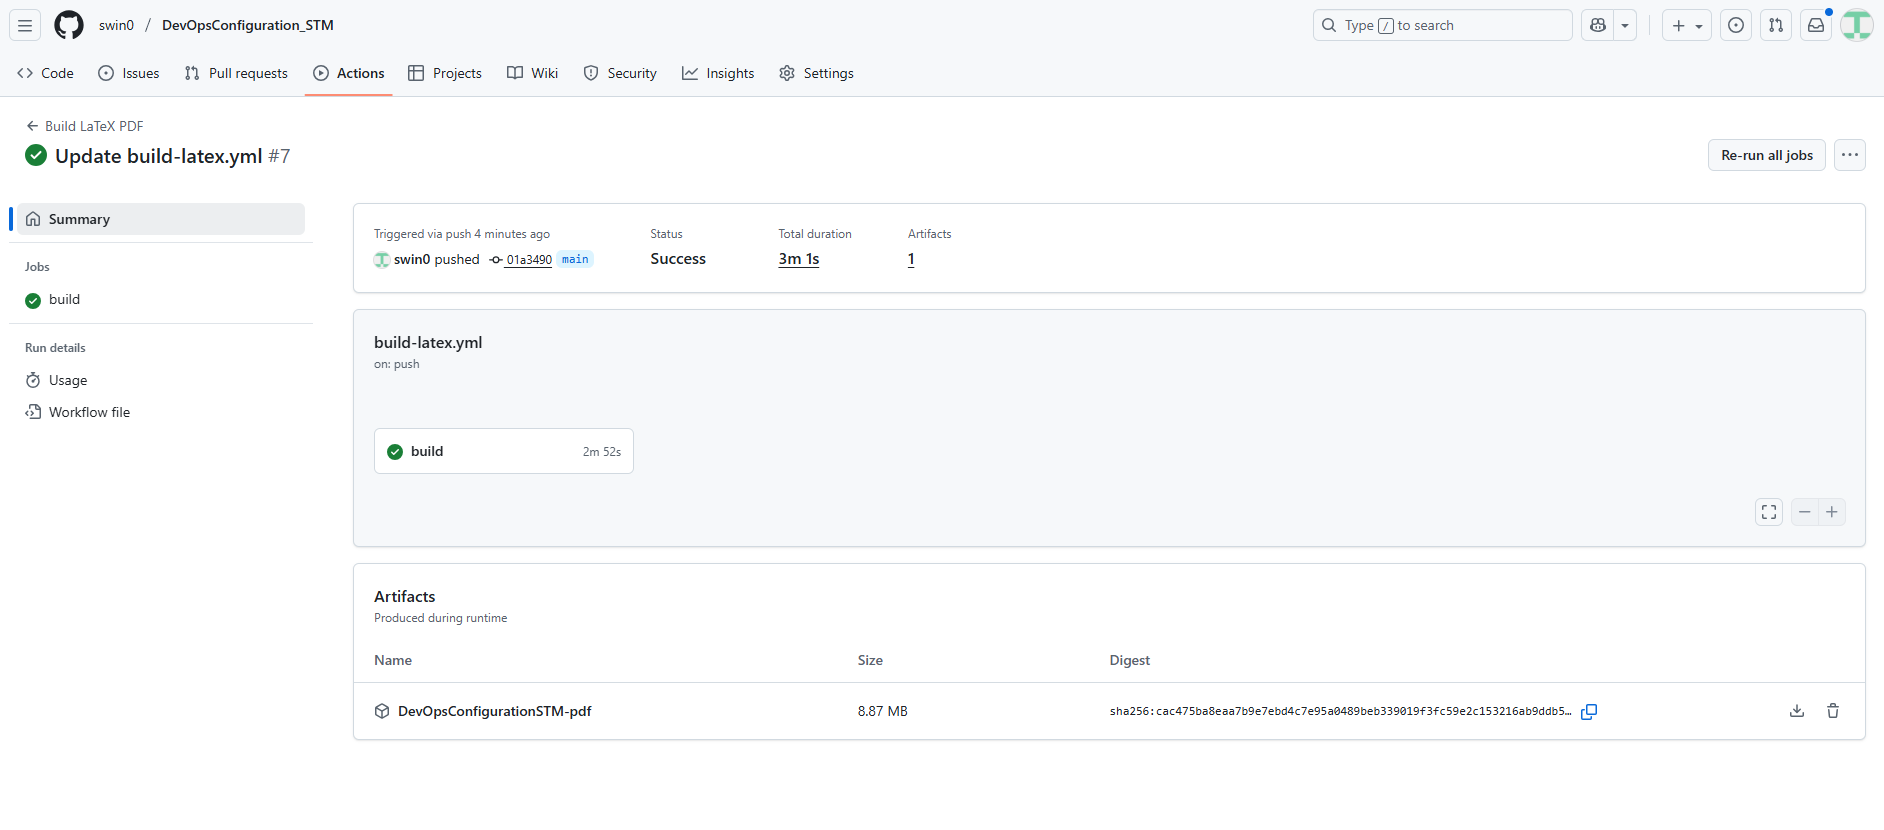
\includegraphics[width=0.9\textwidth]{GitHubActions.PNG}
    \caption{Screenshot of the GitHub Actions build showing successful compilation of the LaTeX document.}
    \label{fig:github_actions_build}
\end{figure}

\section{Compilation and Troubleshooting}

\begin{itemize}
    \item Encountered GitHub Actions issues related to Latexmk and hyperref errors.
    \item Compiled the main document frequently to catch warnings, such as multiply defined labels and hyperref token issues.
    \item Resolved warnings by: \begin{itemize}
        \item Ensuring unique \texttt{\textbackslash label} names for chapters, tables, and figures.
        \item Adjusting float placement with the \texttt{!htbp} specifier.
    \end{itemize}
    \item Verified that all images, minted code listings, and tables rendered correctly.
\end{itemize}

\section{PDF Export}

\begin{itemize}
    \item Downloaded the compiled PDF, which is named itManual.
\end{itemize}
